\section{Technická specifikace}\label{sec:tech}

Tato kapitola popisuje nefunkční (technické) požadavky: konceptuální model domény, odhad velikosti dat a počtu uživatelů, volbu úložišť a technologií, první představu o nasazení a použité vzory. Každá volba je zdůvodněna.

\subsection{Konceptuální model domény}

Model na obrázku~\ref{fig:domain} vychází z \odkaz{sec:vize}{Vize} a z \odkaz{sec:funk}{případů užití}. Obsahuje pouze hlavní třídy, jejich důležité atributy a vztahy s násobnostmi. Metody a technické detaily zatím nejsou uvedeny. Názvy tříd a atributů jsou anglicky, protože stejné názvy se používají v kódu aplikace i v databázovém schématu.

\clearpage
\begin{figure}[H]
  \centering
  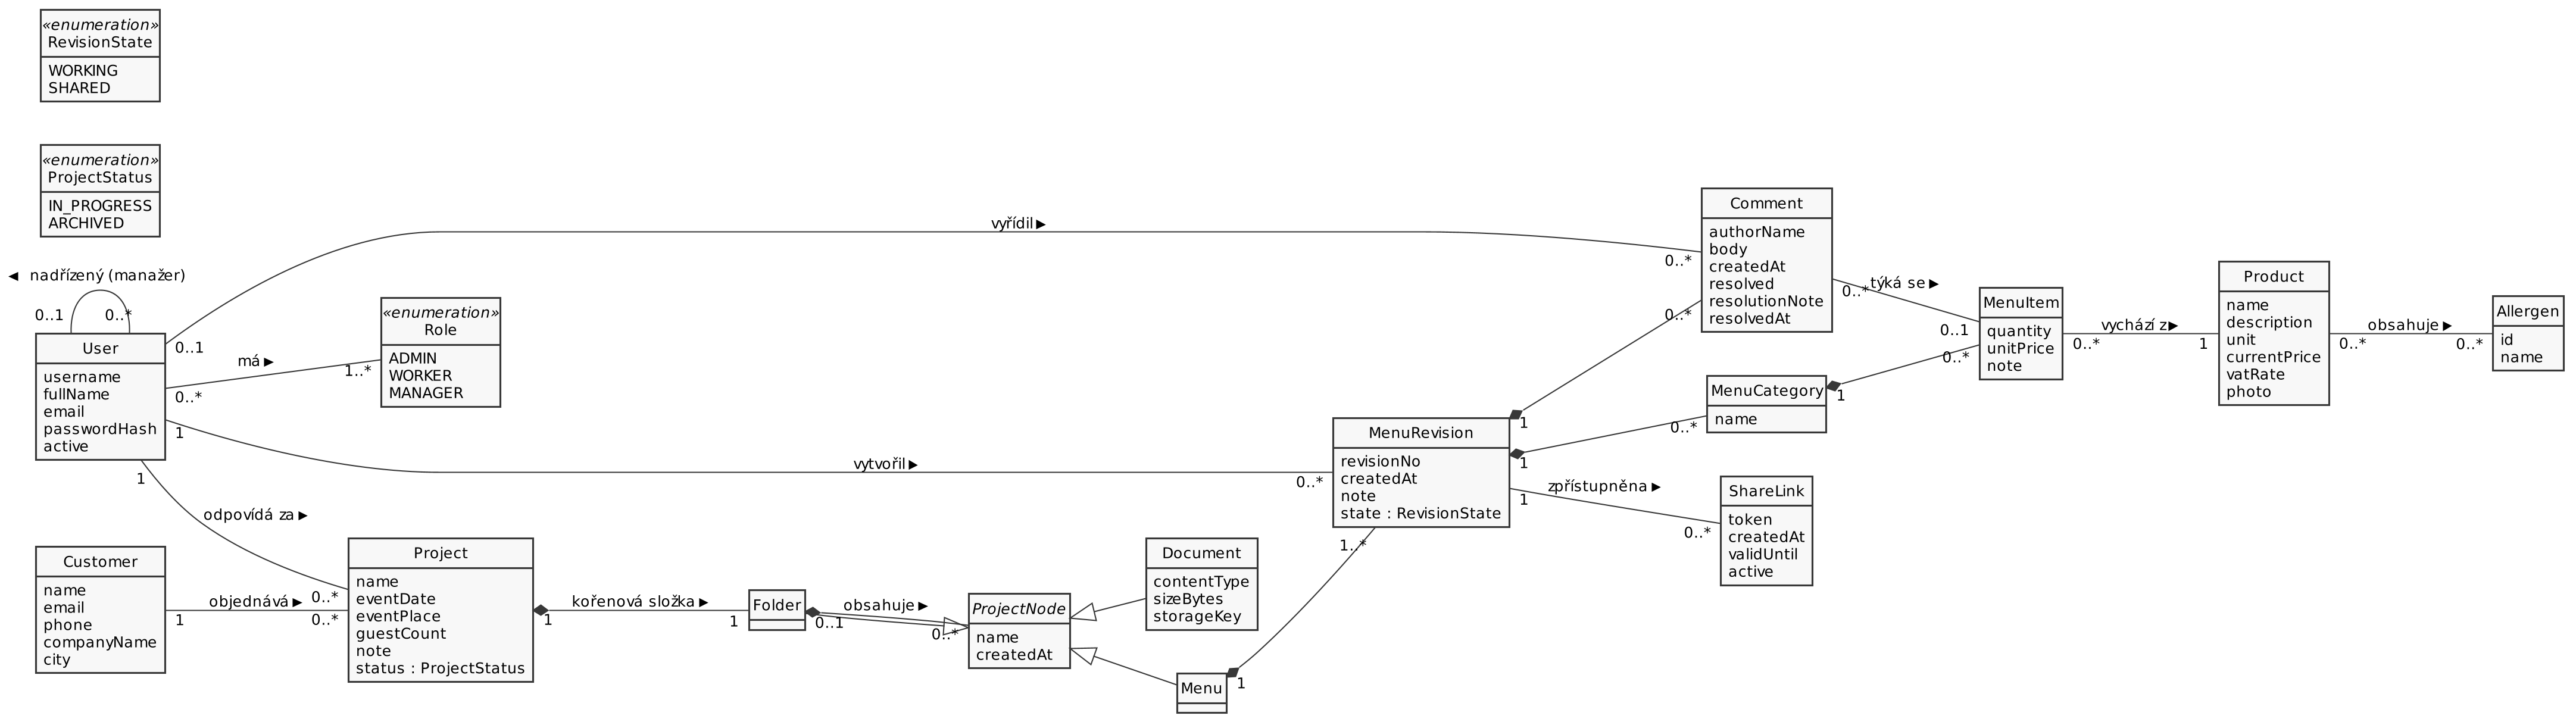
\includegraphics[width=0.85\textheight,angle=90]{domain-model.png}
  \caption{Konceptuální model domény (diagram tříd)}
  \label{fig:domain}
\end{figure}
\clearpage

\begin{description}[itemsep=1pt]
  \item[User, Role] uživatelský účet pracovníka, manažera nebo administrátora. Uživatel má jednu nebo více rolí, které se sčítají. Pracovník u sebe může mít uvedeného nadřízeného (manažera).
  \item[Customer] zákazník, který si objednává catering a může mít více projektů.
  \item[Project] jedna zakázka (akce) s datem, místem, počtem hostů a stavem. Patří jednomu zákazníkovi a odpovídá za ni jeden pracovník.
  \item[ProjectNode, Folder, Document, Menu] obsah projektu uspořádaný do stromu jako jednoduchý souborový systém. Složka obsahuje další složky, dokumenty a menu a každý projekt má právě jednu kořenovou složku.
  \item[MenuRevision] revize menu, které je uzlem ve stromu obsahu. Pracovní revize se při uložení přepisuje. Po sdílení se zákazníkem se revize uzamkne a další úpravy vytvoří novou revizi, takže sdílené revize zůstávají zachovány.
  \item[MenuCategory, MenuItem] kategorie (například předkrmy) a položky revize s množstvím a cenou. Položka vychází z produktu v katalogu. Zjednodušení: revize ukládá u položky množství a jednotkovou cenu, ale název produktu, alergeny a sazbu DPH se čtou z aktuálního katalogu, takže sdílená revize zobrazuje aktuální názvy a alergeny.
  \item[Product, Allergen] katalog pokrmů a nápojů s výchozí cenou, fotografií a alergeny.
  \item[ShareLink] odkaz s omezenou platností, kterým je revize menu zpřístupněna zákazníkovi.
  \item[Výčtové typy] \texttt{ProjectStatus} (IN\_PROGRESS, ARCHIVED), \texttt{RevisionState} (WORKING, SHARED) a \texttt{Role} (ADMIN, WORKER, MANAGER). Typ uzlu stromu (FOLDER, DOCUMENT, MENU) je uložen ve sloupci \texttt{node\_type}, viz Single Table Inheritance. V textu a v uživatelském rozhraní se stavy zobrazují česky: ROZPRACOVANÝ, ARCHIVOVANÝ, PRACOVNÍ a SDÍLENÁ.
  \item[Comment] komentář zákazníka k revizi menu, případně ke konkrétní položce. Pracovník komentář vyřídí s poznámkou a systém si uloží, kdo a kdy jej vyřídil.
\end{description}

\subsection{Odhad počtu uživatelů a typů interakcí}

Podle \odkaz{sec:vize}{Vize} pracuje se systémem v jedné společnosti 10 až 30 interních uživatelů, z toho současně nejvýše přibližně 15 pracovníků v desktopové aplikaci. Společnost má stovky zákazníků a desítky aktivních projektů současně. Pro odhad velikosti dat dále předpokládáme přibližně 300 projektů ročně a uchovávání dat po dobu 5 let.

\begin{table}[H]
\centering
\begin{tabularx}{\textwidth}{lXll}
\toprule
\textbf{Uživatel} & \textbf{Typ interakce} & \textbf{Rozhraní} & \textbf{Současně} \\
\midrule
Pracovník & správa projektů a dokumentů, úpravy menu (časté zápisy, nahrávání souborů do 20~MB) & desktop & do 15 \\
Administrátor & správa uživatelů (občasné zápisy) & desktop & 1 \\
Zákazník & zobrazení nabídky a komentáře (krátké čtení, malé zápisy) & web & do 30 \\
Manažer & prohlížení projektů (pouze čtení) & web & do 3 \\
\bottomrule
\end{tabularx}
\caption{Uživatelé a jejich interakce se systémem}
\end{table}

Role se sčítají a každá odemyká jen svou oblast. Pravidla jsou na jednom místě ve třídě \texttt{AccessPolicy}.

\begin{table}[H]
\centering
\begin{tabularx}{\textwidth}{lXX}
\toprule
\textbf{Role} & \textbf{Desktopová aplikace} & \textbf{Webové rozhraní \texttt{/manager}} \\
\midrule
Pracovník & hlavní okno pracovníka & ne \\
Administrátor & jen administrátorský režim & ne \\
Manažer & přihlášení odmítnuto & projekty vlastních pracovníků \\
Pracovník a administrátor & hlavní okno a přepínač do administrátorského režimu & ne \\
Pracovník a manažer & hlavní okno pracovníka & projekty vlastních pracovníků \\
\bottomrule
\end{tabularx}
\caption{Role a jejich přístup (ostatní kombinace vyplývají ze sčítání rolí)}
\end{table}

Vlastní pracovníci manažera jsou ti, kdo u sebe mají uvedeného tohoto manažera jako nadřízeného. Cizí projekt manažer neuvidí.

Zátěž systému je nízká: jde o desítky požadavků za minutu. Nejnáročnější operací je nahrávání a stahování dokumentů, které ale neprochází databází (viz \odkaz{sec:uloziste}{volba úložiště}).

\subsection{Odhad velikosti dat}

Velikost záznamu je odhadnuta pro kódování Unicode (UTF-8, v databázi znaková sada AL32UTF8). České znaky s diakritikou zabírají 2 bajty, proto je pro text počítáno 2 bajty na znak a výsledek je zaokrouhlen nahoru na stovky bajtů. Například název firmy o 100 znacích zabere až 200~B, adresa místa konání o 200 znacích 400~B. Počty záznamů odpovídají 5 letům provozu jedné společnosti (1\,500 projektů).

\begin{table}[H]
\centering
\small
\begin{tabularx}{\textwidth}{lXrrr}
\toprule
\textbf{Entita} & \textbf{Předpoklad} & \textbf{Záznam} & \textbf{Počet} & \textbf{Celkem} \\
\midrule
User & jméno, e-mail, hash hesla & 400 B & 50 & 20 kB \\
Role + přiřazení rolí & 3 role, 1--2 role na uživatele & 100 B & 100 & 10 kB \\
Customer & jméno, firma (100 zn.), e-mail, telefon, adresa (200 zn.) & 1\,000 B & 1\,000 & 1 MB \\
Project & název, místo (200 zn.), poznámka (300 zn.) & 1\,300 B & 1\,500 & 2 MB \\
ProjectNode -- složka & název, vazby & 300 B & 7\,500 & 2,3 MB \\
ProjectNode -- dokument & název, typ, velikost, klíč v úložišti & 500 B & 30\,000 & 15 MB \\
\textbf{Obsah dokumentů} & průměrně 1 MB (PDF, obrázky) & 1 MB & 30\,000 & \textbf{30 GB} \\
ProjectNode -- menu & název, vazby & 300 B & 3\,000 & 0,9 MB \\
MenuRevision & číslo, stav, poznámka (200 zn.) & 600 B & 12\,000 & 7,2 MB \\
MenuCategory & název, pořadí & 200 B & 60\,000 & 12 MB \\
MenuItem & množství, cena, poznámka (100 zn.) & 400 B & 360\,000 & 144 MB \\
Product & název, popis (500 zn.), cena, jednotka & 1\,200 B & 500 & 0,6 MB \\
Product -- fotografie & zmenšený obrázek JPEG & 100 kB & 500 & 50 MB \\
Allergen + vazby & 14 alergenů, průměrně 2 na produkt & 100 B & 1\,000 & 0,1 MB \\
ShareLink & token, platnost & 300 B & 6\,000 & 1,8 MB \\
Comment & jméno, text do 2\,000 znaků (průměr 500), poznámka k vyřízení (200 zn.) & 1\,600 B & 15\,000 & 24 MB \\
\midrule
\multicolumn{4}{l}{\textbf{Strukturovaná data celkem (včetně fotografií a indexů, cca $\times$1,5)}} & \textbf{cca 400 MB} \\
\multicolumn{4}{l}{\textbf{Obsah dokumentů celkem}} & \textbf{cca 30 GB} \\
\bottomrule
\end{tabularx}
\caption{Odhad velikosti entit pro 5 let provozu jedné společnosti}
\end{table}

Při plánovaném rozšíření na více společností (\odkaz{sec:vize}{Vize}) roste objem lineárně s jejich počtem. Pro 10 společností jde řádově o 4~GB strukturovaných dat a 300~GB dokumentů.

\subsection{Volba úložišť}\label{sec:uloziste}

Systém používá dvě úložiště, ke kterým přistupuje přes oddělené třídy datové vrstvy.

\begin{description}[itemsep=2pt,style=unboxed]
  \item[Relační databáze Oracle] pro všechna strukturovaná data (uživatelé, zákazníci, projekty, strom obsahu, menu a jeho revize, katalog, odkazy a komentáře). Data jsou silně provázaná vazbami a revize menu se musí ukládat atomicky v transakci, což relační databáze s cizími klíči a integritními omezeními zajišťuje přímo. Objem v řádu stovek MB je pro relační databázi malý.

Oracle je ověřený databázový server, který spolehlivě zvládá transakce a souběžnou práci více uživatelů. Do databáze se jako BLOB ukládají i malé fotografie produktů (do 100~kB), aby byl katalog kompletní v jednom místě.
  \item[Souborové úložiště dokumentů] (sdílená složka na aplikačním serveru společnosti) pro obsah dokumentů projektů. Dokumenty jsou na serveru uloženy centrálně, takže je vidí všichni pracovníci a zálohují se na jednom místě, a nezávisí na tom, která stanice je zrovna zapnutá.

Dokumenty zabírají desítky GB, tedy o dva řády více než ostatní data. V databázi by zbytečně zvětšovaly zálohy a zabíraly místo na databázovém serveru. V databázi je u každého dokumentu uložen pouze jeho název, typ, velikost a klíč, pod kterým je soubor uložen ve složce. Soubor lze navíc snadno otevřít běžným programem.
\end{description}

\subsection{Technologická rozhodnutí}

{\footnotesize
\begin{xltabular}{\textwidth}{lXX}
\caption{Technologická rozhodnutí}\\
\toprule
\textbf{Oblast} & \textbf{Volba} & \textbf{Zdůvodnění} \\
\midrule
\endfirsthead
\toprule
\textbf{Oblast} & \textbf{Volba} & \textbf{Zdůvodnění} \\
\midrule
\endhead
Platforma & Java 21 (LTS), OpenJDK, sestavení Maven 3.9 & Aplikace je multiplatformní, což je potřeba, protože společnost používá stanice s Windows i Linuxem. LTS verze má dlouhou podporu. Maven je běžný nástroj pro sestavení a správu knihoven. \\
Desktopové UI & JavaFX 21 (OpenJFX) & Moderní knihovna UI pro Javu s tabulkami, stromy a dialogy, které pracovník potřebuje. Nejde o aplikační framework (MVC apod.), aplikace je psána vlastním kódem. \\
Webové UI & vestavěný HTTP server JDK (\texttt{com.sun.net.httpserver}), stránky generované jako čisté HTML & Zákazník potřebuje jen zobrazit nabídku a odeslat formulář a manažer po přihlášení jen prohlíží projekty. Proto není potřeba webový framework ani samostatný webový server. Server je součástí JDK 21. Aplikace poskytuje stránky přes HTTP. Šifrování HTTPS zajišťuje při nasazení reverzní proxy s certifikátem pro veřejnou doménu společnosti, protože zákazník otevírá odkaz mimo síť společnosti a identifikátor odkazu se nesmí přenášet nešifrovaně. \\
Databáze & Oracle Database 19c nebo novější, při vývoji lokálně Oracle Database 23ai Free & Viz \odkaz{sec:uloziste}{volba úložišť}. Aplikace používá pouze standardní SQL a funkce dostupné od verze 19c, takže poběží na kterékoli novější verzi. \\
Přístup k databázi & JDBC, ovladač Oracle \texttt{ojdbc11} (23.x) & Ovladač podporuje Javu 11+ a databáze Oracle 19c+. Žádné ORM není použito (zákaz Hibernate apod.). \\
QR kód & knihovna ZXing (\texttt{core}) & Malá knihovna pouze pro vykreslení QR kódu s odkazem, nejde o framework. \\
OS stanice & Windows 10/11 (64 bit), Ubuntu 22.04+ nebo jiná distribuce Linuxu, macOS 13+ & Podporované platformy Java 21 a JavaFX 21. \\
Hardware stanice & 4~GB RAM, 1~GB volného místa & Postačuje pro běh JVM s JavaFX. Systém na stanici dokumenty trvale neukládá, kromě souborů, které si pracovník sám stáhne. \\
Aplikační server & Ubuntu Server 22.04 LTS, Java 21, 8~GB RAM, disk alespoň 500~GB & LTS verze systému má dlouhou podporu a server běží bez grafického prostředí. Disk pojme dokumenty několika let provozu s rezervou. \\
Reverzní proxy & nginx 1.18 nebo novější & Ukončuje HTTPS s certifikátem společnosti, bufferuje požadavky a hlídá časové limity klientů. Aplikace sama naslouchá jen na portu 8080 (HTTP). Veřejnosti proxy předává pouze adresy \texttt{/menu/}, přehled manažera (\texttt{/manager}) je dostupný jen ze sítě společnosti (VPN nebo LAN). \\
Prohlížeč zákazníka & Chrome/Edge 120+, Firefox 120+, Safari 17+ (i mobilní) & Stránky používají pouze HTML5 a CSS bez JavaScriptu, fungují na počítači i na telefonu po naskenování QR kódu. \\
Databázový server & Oracle Linux 9, 16~GB RAM, disk 200~GB & Oracle Linux je pro Oracle Database oficiálně podporovaný systém. Paměť i disk mají velkou rezervu proti odhadu velikosti dat. \\
PDF & knihovna Apache PDFBox 3 & Malá knihovna pro vytvoření PDF z revize menu (\ucref{14}), bez dalších závislostí. \\
Plánovač & \texttt{ScheduledExecutorService} z JDK & Denní zneplatnění prošlých odkazů (\ucref{18}) nepotřebuje externí plánovač, stačí standardní třída JDK v serverovém režimu aplikace. \\
Hash hesel & PBKDF2 (\texttt{PBKDF2WithHmacSHA256}) z JDK & Algoritmus je součástí JDK, používá sůl a mnoho iterací, takže hesla nejsou uložena čitelně ani snadno prolomitelná. \\
Server dokumentů & sdílená složka na aplikačním serveru, ke které se stanice připojují přes síť (SMB nebo NFS) & Stejné umístění pro všechny stanice i webové rozhraní, objem desítek GB bez další infrastruktury. \\
\bottomrule
\end{xltabular}}


\subsection{První představa o nasazení}

Aplikace je jeden program v Javě, který obsahuje desktopové i webové rozhraní, aplikační logiku a datovou vrstvu. Na pracovních stanicích běží desktopová aplikace pro pracovníky.

Na aplikačním serveru společnosti běží stejná aplikace ve webovém režimu (třída \texttt{WebMain}) s vestavěným webovým serverem pro zákazníky a manažery a s plánovačem, který jednou denně zneplatní prošlé odkazy (\ucref{18}), a je zde také sdílená složka s dokumenty, kterou používají všechny stanice. Webové rozhraní aplikace naslouchá na portu 8080 (HTTP). Před ním běží reverzní proxy, která přijímá spojení HTTPS na portu 443 a předává je aplikaci. Aplikace (\texttt{catering-is-1.0.jar}) běží jako služba systemd. Webový server a plánovač spouští jen aplikační server. Desktopová aplikace je spustí pouze tehdy, je-li v konfiguraci nastaven příznak \texttt{web.embedded} (výchozí hodnota je vypnuto, zapnout se používá jen při vývoji a ukázce). Databáze přijímá spojení JDBC na portu 1521.

Strukturovaná data jsou uložena na databázovém serveru Oracle. Zákazník a manažer přistupují k systému webovým prohlížečem.

\begin{figure}[H]
  \centering
  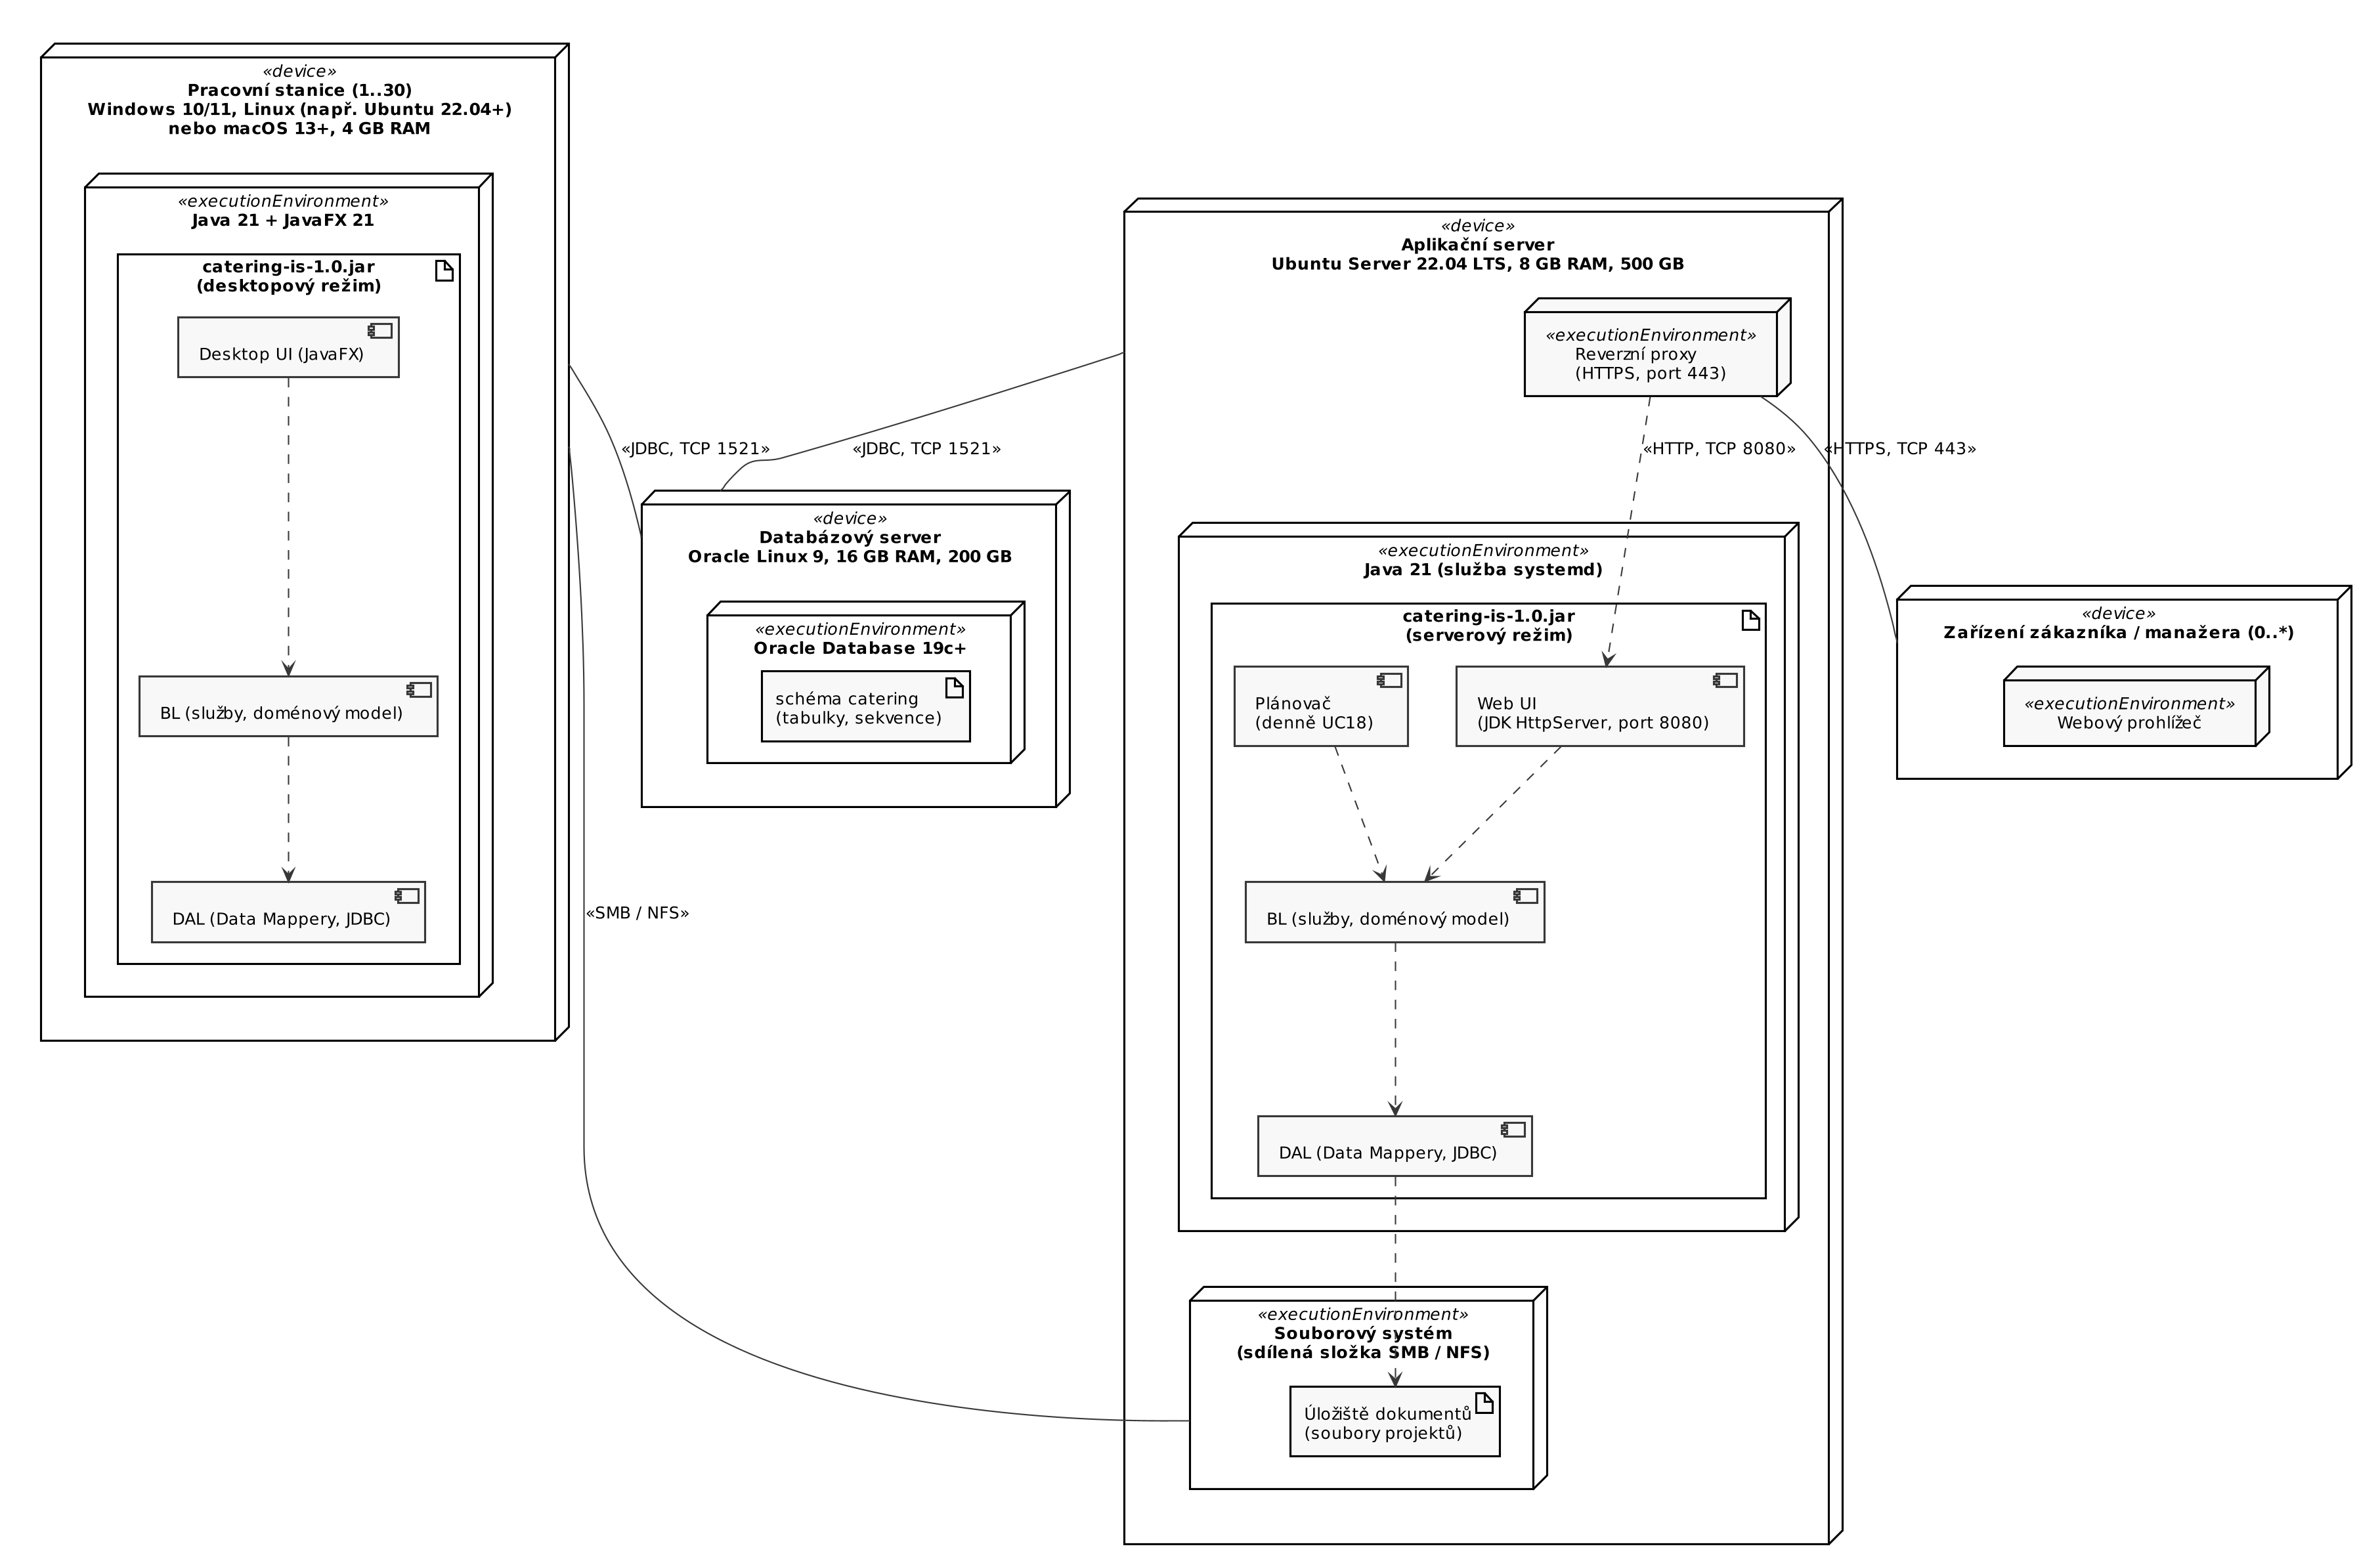
\includegraphics[width=\textwidth]{deployment.png}
  \caption{První představa o rozložení systému}
\end{figure}

\subsection{Použité vzory}

\subsubsection*{Architektonické vzory (vzory pro podnikové aplikace)}

\begin{description}[itemsep=2pt,style=unboxed]
  \item[Vícevrstvá architektura (Layers)] prezentační vrstva (JavaFX, web), aplikační/doménová vrstva a datová vrstva. Závislosti vedou pouze shora dolů, takže obě uživatelská rozhraní používají stejnou aplikační logiku.
  \item[Domain Model] doménové třídy (\texttt{Project}, \texttt{MenuRevision}, \texttt{Folder} \dots) obsahují pravidla, například výpočet ceny menu, kontrolu revize nebo kontrolu jedinečnosti názvu ve složce. Logika tedy není v datové vrstvě.
  \item[Data Mapper] mapper převádí doménové objekty na řádky tabulek přes JDBC a zpět. Mappery jsou \texttt{CustomerMapper} (\texttt{customers}), \texttt{ProjectMapper} (\texttt{projects} a kořenová složka), \texttt{ProjectNodeMapper} (\texttt{project\_nodes}, tedy složky, dokumenty i uzly menu), \texttt{MenuMapper} (\texttt{menu\_revisions}, \texttt{menu\_categories}, \texttt{menu\_items} a \texttt{comments}), \texttt{ShareLinkMapper} (\texttt{share\_links}), \texttt{ProductMapper} (\texttt{products}, \texttt{allergens}, \texttt{product\_allergens}) a \texttt{UserMapper} (\texttt{users}, \texttt{roles}, \texttt{user\_roles}). Doménové třídy o databázi nic nevědí.
  \item[Single Table Inheritance] složky, dokumenty a menu (potomci \texttt{ProjectNode}) jsou uloženy v jedné tabulce \texttt{project\_nodes} se sloupcem \texttt{node\_type} a s odkazem \texttt{parent\_id} na nadřazenou složku. Revize menu jsou v samostatné tabulce. Hierarchie má jen tři potomky s málo vlastními atributy, takže jedna tabulka je nejjednodušší a strom lze načíst jedním dotazem.
  \item[Identity Field, Foreign Key Mapping, Dependent Mapping, Association Table Mapping] identifikátory z databázových sekvencí, vazby přes cizí klíče, kategorie a položky revize ukládané a načítané spolu s revizí, vazba produktů a alergenů přes propojovací tabulku.
  \item[Lazy Load] komentáře revize se nenačítají s revizí v editoru menu. Načtou se samostatným dotazem až při jejich prvním zobrazení (zpracování komentářů, webová stránka nabídky).
  \item[Gateway] přístup k souborovému úložišti dokumentů je skryt za rozhraním \texttt{DocumentStorage}, takže aplikační logika nepracuje přímo se soubory.
  \item[Layer Supertype, Value Object] třída \texttt{DomainObject} je společný předek entit s identifikátorem. Třída \texttt{Money} je neměnná peněžní částka porovnávaná podle hodnoty.
  \item[Special Case, Service Stub] třída \texttt{UnknownShareLink} zastupuje neexistující odkaz, takže služba nekontroluje \texttt{null}. Třída \texttt{InMemoryDocumentStorage} nahrazuje úložiště dokumentů v testech.
  \item[Optimistic Offline Lock] souběžná změna revize se pozná podle stavu a času posledního uložení. Tabulka nemá sloupec s verzí.
  \item[Transakce] uložení revize menu včetně kategorií a položek a sdílení revize probíhá v jedné JDBC transakci. Transakci řídí aplikační služba přes sdílené připojení \texttt{Database} (commit, při chybě rollback), mappery samy transakci neukončují. Pokud se při nahrávání dokumentu nepodaří zapsat záznam do databáze, služba soubor z úložiště smaže.
\end{description}

\subsubsection*{Návrhové vzory GoF}

\begin{description}[itemsep=2pt,style=unboxed]
  \item[Composite] \texttt{Folder}, \texttt{Document} a \texttt{Menu} mají společného předka \texttt{ProjectNode} a složka obsahuje kolekci uzlů. Strom projektu se tak prochází jednotně, například při zobrazení v JavaFX stromu nebo při kontrole, zda je složka před smazáním prázdná (\ucref{19}).
  \item[Factory] jedna továrna vytváří mappery a úložiště dokumentů podle konfigurace (připojení k databázi, cesta ke složce). Zbytek aplikace pracuje jen s rozhraními.
  \item[Singleton] jedna instance poskytovatele databázových připojení (\texttt{Database}), kterou sdílejí všechny mappery. Připojení JDBC otevírá pro každou transakci zvlášť a drží je pro aktuální vlákno.
  \item[Facade] aplikační služby tvoří jednoduché rozhraní nad doménou a datovou vrstvou. Desktopové i webové UI volají pouze tyto služby. \texttt{ProjectService} obsluhuje projekty, \texttt{CustomerService} zákazníky, \texttt{DocumentService} složky a dokumenty, \texttt{MenuService} menu a revize, \texttt{MenuExportService} export do PDF, \texttt{CatalogService} katalog produktů, \texttt{SharingService} sdílení, komentáře a denní zneplatnění odkazů (\ucref{18}), \texttt{AuthService} přihlášení a \texttt{UserService} uživatele.
  \item[Factory Method] abstraktní třída \texttt{NodeCreator} provede společné kroky vytvoření uzlu stromu a potomci \texttt{FolderCreator}, \texttt{MenuCreator} a \texttt{DocumentCreator} určí, jaký uzel vznikne.
  \item[Strategy] rozhraní \texttt{PriceStrategy} s implementacemi \texttt{PriceWithoutVat} a \texttt{PriceWithVat} určuje, zda se ceny zobrazují bez DPH nebo s DPH.
  \item[Observer] \texttt{MenuRevision} oznamuje změny posluchači \texttt{MenuRevisionListener}, kterým je editor menu.
  \item[Command] každá úprava menu je objekt s rozhraním \texttt{MenuEditCommand}. Třída \texttt{MenuEditor} je spouští a umožňuje vrátit poslední úpravu (Zpět).
\end{description}
